$y=\ln(e^x-1)/(e^x+1)$ desde $x=2$ a $x=4$.

\nopagebreak
\begin{align*}
y = \ln(e^x-1) - \ln(e^x+1). \\
y' = \frac{e^x}{e^x-1} - \frac{e^x}{e^x+1} = \frac{e^x(e^x+1) - e^x(e^x-1)}{e^{2x}-1} = \frac{2e^x}{e^{2x}-1}. \\
1+(y')^2 = 1 + \frac{4e^{2x}}{(e^{2x}-1)^2} = \frac{(e^{2x}-1)^2 + 4e^{2x}}{(e^{2x}-1)^2} = \frac{(e^{2x}+1)^2}{(e^{2x}-1)^2}. \\
L &= \int_{2}^{4} \frac{e^{2x}+1}{e^{2x}-1} \, dx = \int_{2}^{4} \coth(x) \, dx \text{ (aprox)}. \\
\text{Exacto: } \int \frac{e^{2x}+1}{e^{2x}-1} dx = \ln(e^{2x}-1) - x. \\
L &= [\ln(e^{2x}-1) - x]_{2}^{4} \\
&= (\ln(e^8-1) - 4) - (\ln(e^4-1) - 2) \\
&= \ln\left(\frac{e^8-1}{e^4-1}\right) - 2 = \ln(e^4+1) - 2
\end{align*}

\[
\boxed{\displaystyle \ln(e^4+1) - 2}
\]

\begin{center}
    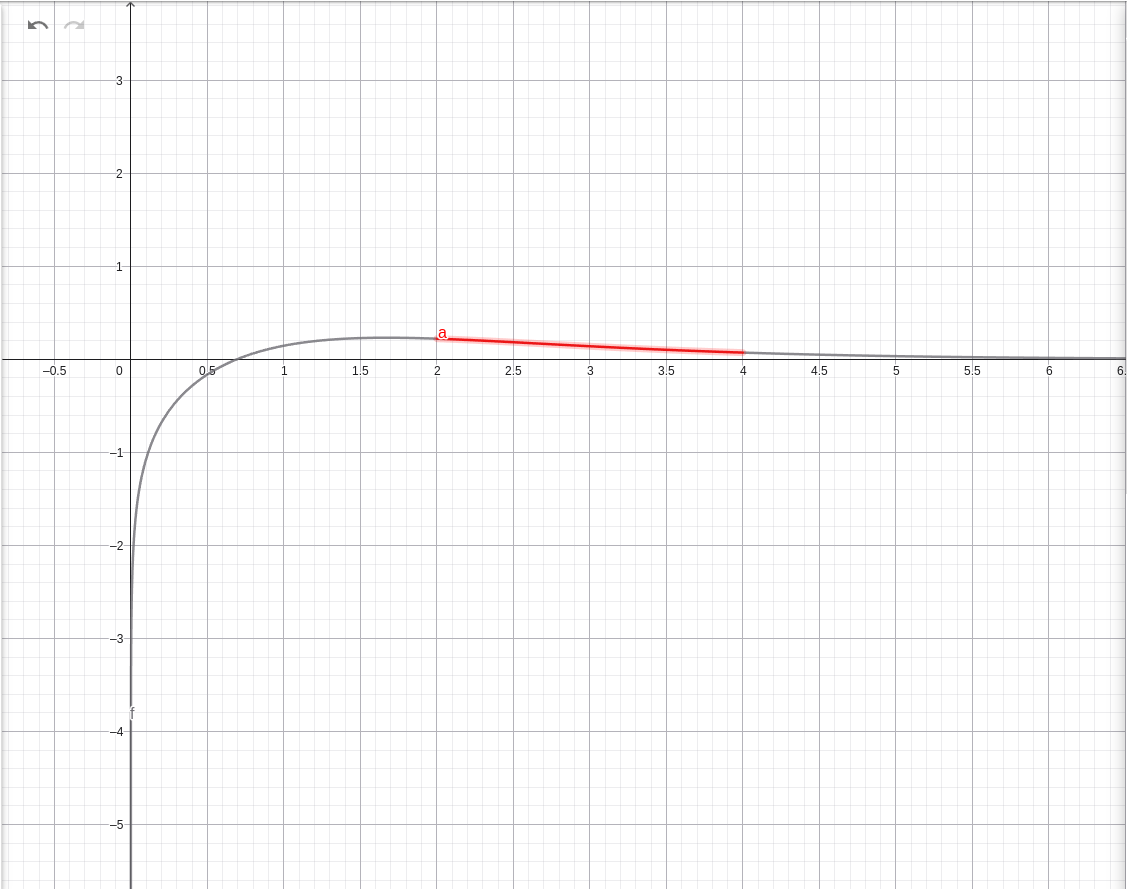
\includegraphics[width=0.5\textwidth]{Graficas/ejer48.png}
\end{center}
